\begin{figure}[!t]
\centering
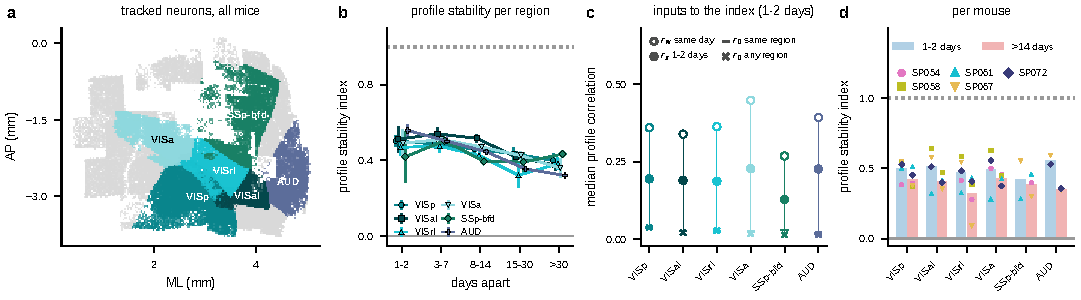
\includegraphics{regions.pdf}
\caption{\textbf{Profile stability per cortical region.} Profile stability index (Fig.~\ref{fig:main}b), computed on the tracked neurons of each region, with chance $r_0$ from a partner of the same region and FOV. Region colours are shades of the Allen atlas colours: teal for visual areas, green for SSp-bfd, and slate for AUD (whose Allen teal would clash with the visual areas). Dotted line, same-day baseline (1); grey line, chance (0); dots, mice (colours as in Fig.~\ref{fig:main}); bars, mean over mice; error bars, s.e.m.\ over mice.
\textbf{a}~Tracked neurons of all mice in a dorsal view of the CCF (ML, AP), coloured by region; other regions in grey.
\textbf{b}~Index against days apart, per region.
\textbf{c}~Inputs to the index at 1--2 days apart (medians, mean over mice). $r_w$: same day, even vs.\ odd trials (open). $r_x$: across days (filled). $r_0$: random partner of the same region (bar) or of any region (cross). The index is $(r_x-r_0)/(r_w-r_0)$.
\textbf{d}~Index at 1--2 days (blue bars) and $>$14 days apart (red bars); symbols, individual mice.}
\label{fig:regions}
\end{figure}
